
\section{Introduction }\label{compression:introduction}



Mammography is the sole screening method recognized by the European Commission for women aged 50-69 years. It's morphological method enable examination of the breast in its entirety and offer a high sensitivity for early-stage tumours. However, the mammographic exam is knew to be awkward and  unpleasant for the patient,  the main source of discomfort lying in it's operating principle. The perceived pain is related to the breast compression between the image receiver and the compression paddle.

For such a standard and wide-used procedure good conditions and patient comfort should be ensured. Therefore a study on the relevance of breast compression methodology in mammography is of a potential interest. In the next chapters, a numerical simulation tool enabling the characterization of existing breast compression techniques in terms of patient comfort id developed. 
 The latter would serve to build an optimal compression paddle, and therefore increase the adherence to breast cancer screening. 




In this purpose, MR images of two subjects are used to create patient specific finite elements breast models. The mechanical behavior of soft tissues under compression is computed for both subjects and for both paddle designs. The perceived pain for a given paddle design is quantitatively characterized by contact pressure, internal stress and strain distributions. After compression, three sets of macrocalcifications are inserted into breast volumes. The latter are then subject to a Monte-Carlo based simulation (CatSim8) enabling to simulate the image acquisition of the compressed breast with a mammography system. Then, the diagnosis quality is assessed by measuring the signal-difference-to-noise-ratio (SDNR), signal-to-noise-ratio (SNR) and the average glandular dose (AGD). 
\clearpage 
\section{Breast compression: overview }\label{section:compression:stateoftheart}

{\color{darkblue}
-Describe breast positioning and compression (Groot) \\
-Describe today\'s  compression standards: force-thickness relation; thickness- AGD; force/thickness and pain relation;  Pressure standardized mammography.}
\subsection{Mammographic positioning} \label{subsec:mammographicpositioning}

During mammography, a qualified radiologic technologist positions the breast of the patient between the stationary bucky (X-ray detector hausing) and a movable paddle. A routine mammographyc exam consists of two views: cranio-caudal (CC) and mediolateral oblique (MLO) projections. The views are complementary and provide a complete image of the entire breast. However, sometimes special view can be required  to confirm or reject suspicious findings \citep{groot_towards_2015}. 

In a regular workflow, the breast compression is performed in the up-right body position. In the CC view the breast is placed on the bucky , which is initially positioned at the inframammary folder level or a few cm higher depending on breast mobility in the corresponding direction. Then the technologist lowers the compression paddle using a foot switch and gently pull the breast onto the bucky to correctly position the breast and to maximize the amount of projected tissues. In the MLO view, the bucky is rotated to an angle between 40 to 55 degrees. The woman rests the lateral oblique site of her breast against the bucky. In this view the pectoral muscle is located between the detector the compression paddle; As the muscle is stiffer then the breast tissues , the woman have to stay relaxed in order to have better breast flattening. When lowering the compression paddle, the technologist have to pull the breast up and forward to prevent drooping of the breast, and again smoothen out any skin folds.

The mammography devices are equipped with paddle position and force sensors to measure ans display the compressed breast thickness and the amount of force applied to the breast.


\begin{figure}[!h]
\centering
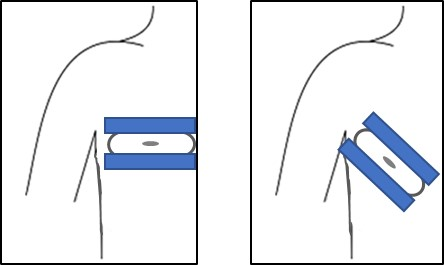
\includegraphics[width=0.5\textwidth,keepaspectratio]{figures/cc_mlo_view.jpg} 
\caption{left: cranio-caudal breast compression; righ - mediolateral oblique breast compression }\label{fig:cc_mlo_view}
\end{figure}


\subsection{Compression mechanics} \label{subsec:compressionmechanics}
 \cite{de_pain_2015} studied the breast compression cycle, according to the authors the compression cycle is characterized by two phase: flattening and clapping. During the flattening phase, the breast is gradually  deformed by increasing the compression force, the deformation lasted  $7.5 \pm 2.6$. By contrast, during the clamping phase which last approximately $12.8 \pm 3.6$ , the compression paddle is immobilized holding the breast in a stationary position. 
\begin{figure}[!h]
\centering
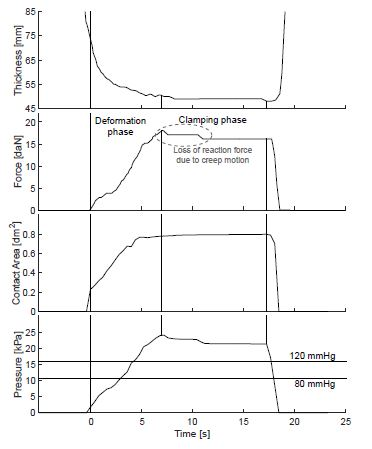
\includegraphics[width=0.7\textwidth,keepaspectratio]{figures/breast_compression_cycle.jpg} 
\caption{A typeical breast compression cycle. Reproduced from \cite{groot_towards_2015}}\label{fig:breast_compression_cycle}
\end{figure}

Figure \ref{fig:breast_compression_cycle} shows a typical compression cycle for a CC breast compression. One can see that during the compression paddle the breast thickness and contact area evolve non-linearly and remains constant during the clamping phase. The compression force and pressure increase quasi-linearly, however in the first $10s$ of the clamping phase they slightly decrease. This may be explained by breast volume changes because of the viscous effusion of blood and lymph into the central systems. 

Figure \ref{fig:thickness_force_patterns_groot} shows the relation between breast thickness and compression force  depending on breast size and firmness. One can see that, for a larger breast size higher compression force is needed, but the overall behavior remains the same. For similar breast sizes, the final compression force stay within the same range, however a firmer breast will reach faster the limiting value of breast thickness resulting in a direct increase of the compression force.
\begin{figure}[!h]
\centering
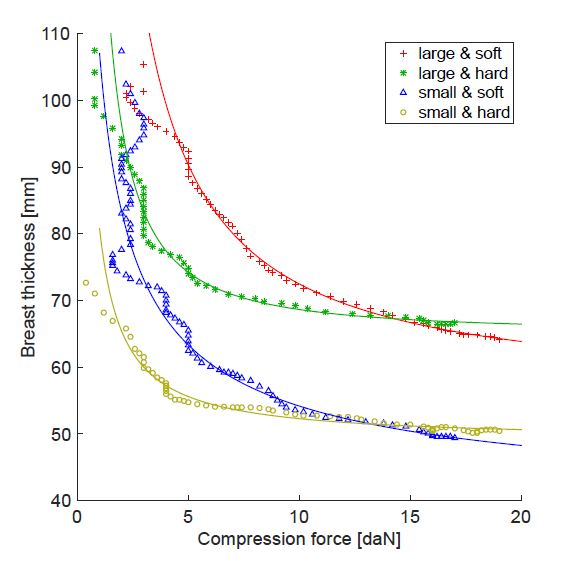
\includegraphics[width=0.7\textwidth,keepaspectratio]{figures/thickness_force_patterns_groot.jpg} 
\caption{Characteristic breast flattening curve as function of the applied force. Reproduced from \cite{groot_towards_2015}}\label{fig:thickness_force_patterns_groot}
\end{figure}

\subsection{Compression paddle designs} \label{section:compressionpaddlesdesign}

In addition to the large and small standard paddles, many
compression paddles of varying size and shape are included
with each mammography unit. Although each paddle has specific
indications, using the paddles creatively may facilitate the
positioning process

 The technologist gradually compresses the breast in order to even out the breast thickness and to spread out the soft tissues. Nowadays, two types of compression paddles are widely available: rigid compression paddles (RCP) and flex compression paddles (FCP). 


The RCP is fixed to its frame and is constrained to move in the up-down direction. This paddle has some flexibility because of material mechanical properties and can slightly bend when compressing the breast, while remaining globally flat and parallel to the image receptor. On the other hand, the FCP is attached to its frame by rotational joints and therefore, presents an additional rotational degree of freedom enabling the paddle to tilt with respect to the image receptor plane (Figure 3.c). 

\begin{figure}[!h]
\centering
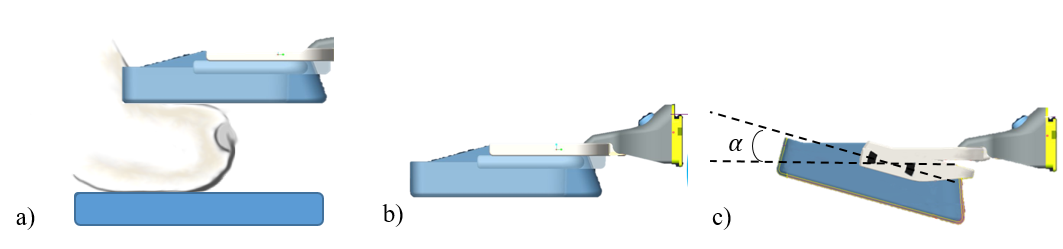
\includegraphics[width=0.9\textwidth,keepaspectratio]{figures/compressionpaddles.png} 
\caption{Breast compression between the paddle (up) and the receiver (down): a) Rigid paddle; b)Flex paddle with flexion angle $\alpha$}\label{fig:compressionpaddles}
\end{figure}

\section{Pain and discomfort}
\section{Image quality and average glandular dose}


\section{Discussions and Conclusion}\label{section:compression:conclusion}

Great strides in positioning are evident in the field today.
We are imaging more tissue than before, but not without
experiencing some drawbacks. For example, imaging greater
amounts of posterior tissue in thick breasts can reduce the
amount of compression in the anterior breast—possibly
obscuring a small anterior cancerous tumor. The technologist
has the critical job of applying positioning methods using
common sense, as in the previous case—an additional third
projection to better compress the anterior tissue may be necessary.
Use of available tools, such as the American
Mammographics S.O.F.T. Paddle or Hologic FAST Paddle
may be another option.